\chapter{Architecture}
\label{chapter:architecture}

\section{Introduction}
\label{section:introduction}
In this chapter the tools used for implementation and the basic architecture are explained. First the used programming language and framework are introduced, then how the different parts of the learning environment work together and finally some frequently used mechanisms are explained.

\section{TypeScript}
\label{section:typescript}
JavaScript had its publication in 1996, it is a dynamically typed scripting language and is intended to be used in browsers to extend the possibilities of HTML and CSS. It can dynamically manipulate HTML and CSS, validate user data, send and receive data without reloading the page and much more. JavaScript used in browsers is run on client-side i.e. the workload is shifted from the provider of the web application to the client computer \cite{Javascript}. 

TypeScript extends JavaScript by providing type safety and concepts such as interfaces, methods signatures, interfaces, enumerations and tuples. It provides a way to describe what type a variable has and helps to catch errors before the code is run. The type safety is assured during compilation from TypeScript to JavaScript \cite{Typescript}.

\section{Vue.js}
\label{section:vuejs}
Vue.js is a reactive, client-side JavaScript web framework developed by Evan You and its community starting in 2014. It is an alternative to Angular and React and was supposed to be a lightweight version of Angular. Vue.js is also based on reusable components, each having its own HTML, JavaScript and CSS. The reactivity system of Vue.js allows changes made to the application data to be automatically reflected in the browser.
When the development of this project started in November 2020, Vue.js version 3 was already published. However, Vue.js version 2 is used in this project, because the ecosystem has not caught up yet and many libraries only work with version 2 at the moment \cite{Vue}.

\subsection{Components}
Components are named reusable Vue.js instances and have the advantages that the structure, functionality and style of an element is implemented once and can then easily be used multiple times. Therefore, each component has a parent (except from the root component) and possibly multiple child components forming a tree structure. 

Everything in Vue.js is a component, but not everything is a page. A page needs a route e.g. \code{/settings} and components with a route are called views. 

Mixins can be used to reuse functionality over different Vue.js components. When a component uses a mixin, all functionalities of the mixin are mixed into the component \cite{Vue}. 

\subsection{Communication Between Components}
Vue.js supports bi-directional communication between parent and child components. The communication takes place via properties from the parent to the child and via events from the child to the parent. Properties are custom attributes that pass data from the parent to the child component. Events are emitted by a child component, can carry data and a parent can listen and react upon receiving an event from a child component \cite{Vue}.

\subsection{Best Practices}
The following list represent the best practice that were applied in this project. To see examples for each best practice visit the Vue.js style guide  \cite{VueStyleGuide}.

\section{Basic Functionality}
\label{section:basicFunctionality}

\subsection{Home Screen}
The home screen is a view and is the first page seen when visiting the learning environment (figure \ref{fig:homepage}). For each available exercise there is a card with an image to illustrate the exercise and its title. The basic ideas for the images are taken from the text book, but most of the time needed some simple image manipulation to make it represent the task reasonably.

\begin{figure}[h]
    \centering
    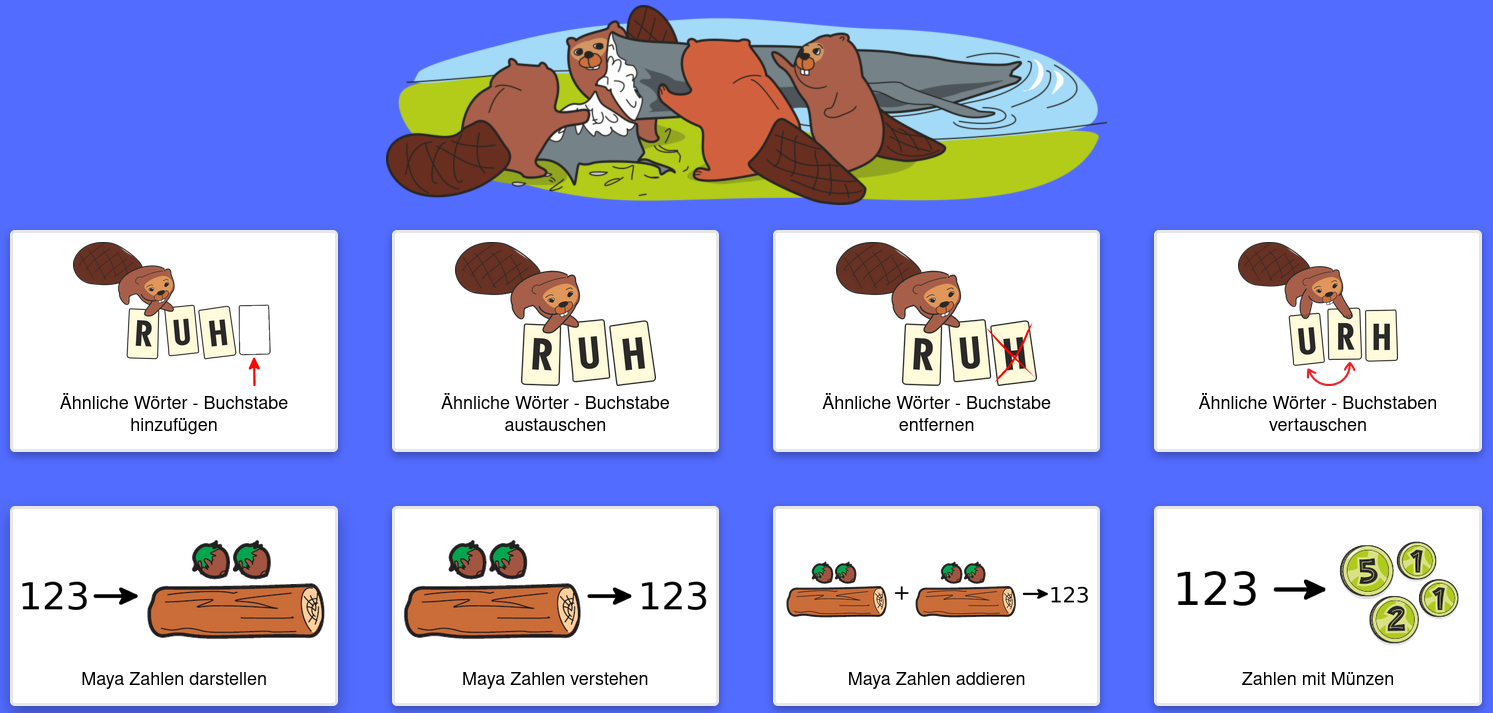
\includegraphics[width=1.0 \columnwidth]{figures/homepage.png}
    \caption{Homepage excerpt} 
    \label{fig:homepage} 
\end{figure}

\subsection{Game Mixin and Game Interface}

\subsection*{Game Mixin}
All exercises use the \code{GameMixin} containing the functionality on starting and evaluating an exercise. Additionally, a function to generate a random number exists to mock random number generation in tests. More on that in \nameref{section:testing}.

\subsection*{Game Interface}
Each exercise implements the \code{GameInterface}. This ensures that specific functionalities, like starting and evaluating the exercise, are implemented and can be used in the \code{GameMixin}.

%TC:ignore
\begin{lstlisting}[language=TypeScript,caption={GameInterface},label={lst:gameInterface}]
interface GameInterface {
    isInitialized(): boolean;
    start(): void;
    isCorrect(): boolean;
}
\end{lstlisting}
%TC:endignore

\subsection{General Purpose Components}
\label{subsection:generalPuprposeComponents}
The following presented components are components that are crucial or heavily reused. Most of them are part of the user interaction system since all exercises need some kind of user interaction elements.

\subsection*{Game}
The Game component is the crux of the matter
\TODO{explain game component}

\subsection*{Event Bus}
Sometimes components are not in a direct parent-child relationship and still need to communicate. This can be achieved by passing properties and emitting events. Downside of this approach is the quick loose of clear structure. To tackle this problem, one can use an event bus. 
The event bus is a Vue.js instance that allows to emit an event in one component and listen for that event on another component. To use the event bus, a component simply needs to import the instance and can emit or listen for events on the usual way. In this project, the event bus is used between the \nameref{subsection:gameButtons} and each exercise.

\subsection*{Game Buttons}
\label{subsection:gameButtons}
Every exercise needs a \textit{check exercise} and a \textit{next exercise} button (figure \ref{fig:gameButtons}). The former is used to validate a given solution and the latter to load the next exercise.

\subsection*{Undo Button}
The \textit{undo} button simply restores the current exercise initial conditions, so one can retry it again.

\begin{figure}[h]
    \centering
    \begin{subfigure}[b]{0.4\textwidth}
        \centering
        
\includegraphics[width=\textwidth]{figures/game_buttons.png}
        \subcaption{}
        \label{fig:gameButtons} 
    \end{subfigure}
    \begin{subfigure}[b]{0.4\textwidth}
        \centering
        
\includegraphics[width=0.2\textwidth]{figures/undo.png}
        \subcaption{}
        \label{fig:undo} 
    \end{subfigure}
    \caption{Game buttons \ref{fig:gameButtons} and undo button \ref{fig:undo}}
\end{figure}

\subsection*{Trashcan Button}
The \textit{trashcan} button (figure \ref{fig:trashcan}) is an area where elements can be dropped to remove them. For example when pupils are asked to remove a letter from a word, they can either drag the letter to this area and drop it or first click on the letter and then on the \textit{trashcan} button to remove it.

\subsection*{Difficulty Level Buttons}
Some exercises have multiple difficulty levels (figure \ref{fig:difficultyLevels}). For those exercise the \textit{difficulty level} buttons are used to change the difficulty level. This component gives the possibility to choose from up to three different difficulty levels indicated by an increasing amount of beavers on the button and a title that is showed on hover.

\begin{figure}[h]
    \centering
    \begin{subfigure}[b]{0.3\textwidth}
        \centering
        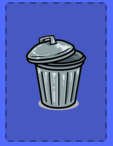
\includegraphics[width=0.35\textwidth]{figures/trashcan.png}
        \subcaption{}
        \label{fig:trashcan} 
    \end{subfigure}
    \begin{subfigure}[b]{0.5\textwidth}
        \centering
        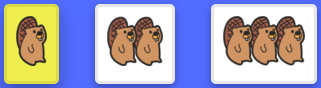
\includegraphics[width=\textwidth]{figures/difficulty_level.png}
        \subcaption{}
        \label{fig:difficultyLevels} 
    \end{subfigure}
    \caption{Trashcan button \ref{fig:trashcan} and difficulty level buttons from easy to hard \ref{fig:difficultyLevels}}
\end{figure}

\subsection*{Tutorial Button}
To introduce an exercise to the pupils the title of the exercise and a short instruction is not enough. Therefore, for each exercise there is a detailed explanation and a tutorial video (figure \ref{fig:tutorialButton} and figure \ref{fig:tutorialExample}). The tutorial video shows an example run giving first a wrong solution, then restarting the exercise and finally, giving the correct solution.

The tutorial videos were recorded by a screen capture tool and the mouse movement on how to solve the exercise is done programmatically. The main reason for this is that the tutorial video needs to be redone whenever the user interface changes. With this, rerecording the tutorial video is much more convenient. Another reason is that moving the mouse by hand to solve the exercise introduces a jitter to the mouse movement and might be irritating. The tutorial on the other hand should show clearly and without any hesitation the way on how to solve the exercise. Since this cannot be done by an average human being, the mouse movement is done programmatically. 

Each graphical element part of the exercise has an ID and one can give a list of IDs that should be visited in a run. The tutorial video then shows a mouse visiting and interacting with these graphical elements and demonstrates how to solve the exercise. 

\begin{figure}[h]
    \centering
    \begin{subfigure}[b]{0.25\textwidth}
        \centering
        
\includegraphics[width=0.5\textwidth]{figures/tutorial_button.png}
        \subcaption{}
        \label{fig:tutorialButton} 
    \end{subfigure}
    \begin{subfigure}[b]{0.7\textwidth}
        \centering
        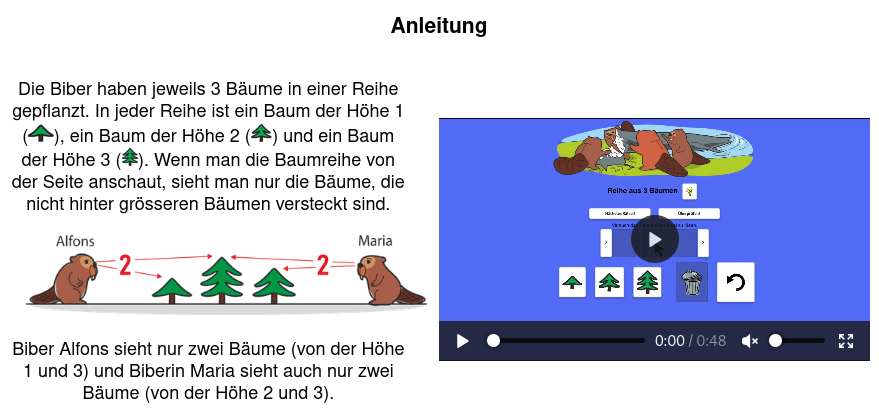
\includegraphics[width=\textwidth]{figures/tutorial_example.png}
        \subcaption{}
        \label{fig:tutorialExample} 
    \end{subfigure}
    \caption{Tutorial button \ref{fig:tutorialButton} and tutorial of the row of trees exercise \ref{fig:tutorialExample}}
\end{figure}